\chapter{Introduction}
This chapter aims to familiarize the user with the domain and some of its challenges. The first sections will explain the purpose and motivation of our project. Next we describe our research questions and how we aim to answer them.  Lastly we present relevant research already conducted in the field.

\section{Purpose}
The purpose of the project is to explore the possibility of creating a mobile biofeedback system through the use of a smartphone and cheap mass produced peripherals. The smartphone will act as a hub, while sensor based peripherals attached to the user will gather information. The information will be processed by the smartphone, and appropriate feedback will be provided to the user; feedback will be provided by using vibration and audio. By acknowledging the feedback the user can improve his or her gait, and reduce the likelihood of a fall.

\section{Motivation}
Falls are a major health hazard among the elderly population (age \textgreater{} 65) \cite{fallsHealthHazard}, in addition to being an obstacle for physical activity and independent living. Physical activity can be an important instrument in improving the quality of life and preventing future disabilities for the elderly\cite{physicalActivity}. A third of all elders that experience a fall, develop a fear of falling \cite{fearOfFalling}. Fear of falling causes general anxiety and avoidance of physical activity. Long term consequences result in social isolation, physical deterioration and reduced quality of life.\cite{physicalAvoidance} %Skrive noe om hvor mye det koster staten å passe på de eldre?

Between 30\% and 60\% of the elder population will experience at least one fall per year, and 10-20\% of these will result in an injury, hospitalization or death \cite{fallStatistics}. For the independent elder population it is even more crucial that a fall can be avoided and the proper authorities can be alerted if a fall does occur. In the case of a serious fall a slow response time might increase the likelihood of permanent damage or death\cite{personHomeDeath, dangerousFallHome}.

Technological progress has made it easy and affordable to incorporate sensors into devices in order to provide a better or more entertaining user experience. Accelerometers, gyroscopes and GPS are an expected feature in today's smartphones. Newer phones include even more advanced sensory such as Barometers, and Proximity Sensors.

Motion based games and game controllers have been a trend in the gaming industry for the last 8 years. It started with the Nintendo Wii, but Microsoft and Playstation followed quickly with their own motion based technology, Kinect and PS Move respectively. The competition to offer the best product on the market has made motion sensing more powerful, and mass production has made it affordable.

\section{Research questions}
The primary goal is to explore the possibility of a mobile biofeedback system through the use of mass produced off the shelf products. An Android smartphone will function as the central hub for the system. Game controllers with motion detecting capabilities will be attached to the user in key locations and Bluetooth will be used to transmit sensor data to the smartphone. The smartphone will process and compute data and act as a user interface. The system will provide the user with feedback through audio and vibration. The smartphone will be responsible for the audio feedback, while the game controller will provide feedback through vibration. Our primary goal leads us to several research questions which we aim to answer in this paper.

\begin{figure}[h!]
  \centering
    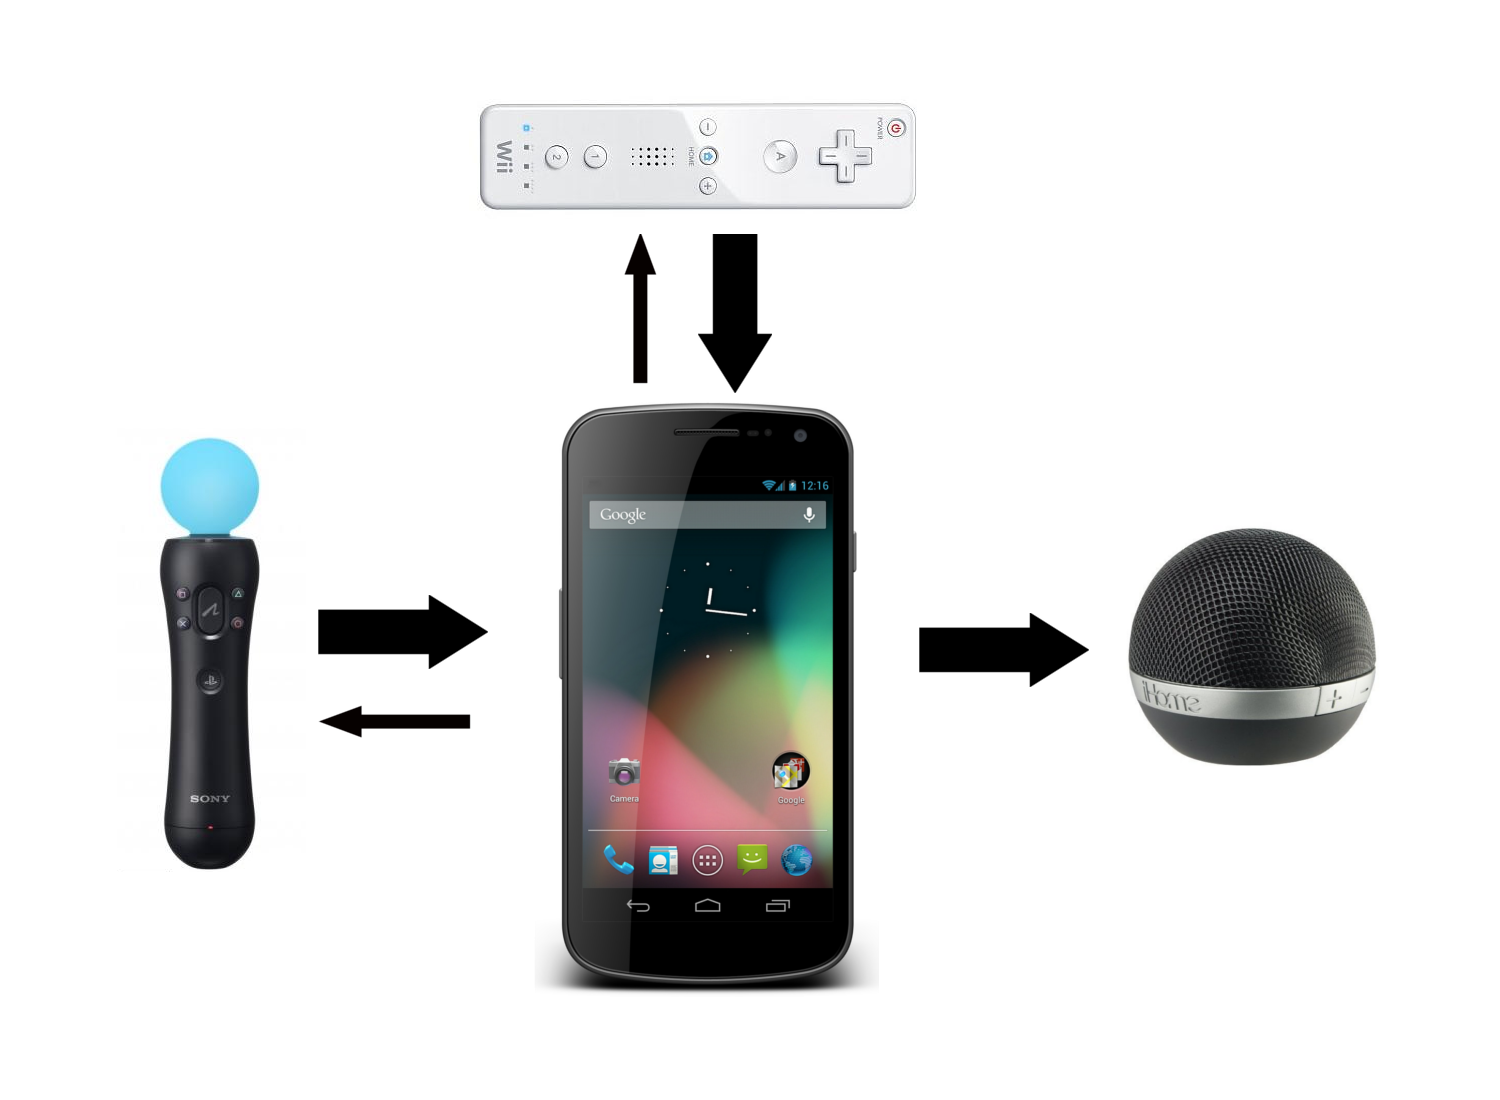
\includegraphics[width=.80\textwidth]{hub.png}
    \caption{\footnotesize A conceptual image of the hardware involved in a mobile biofeedback system. Arrows represent the information flow, and the thickness represent the intensity.}
\end{figure}

\begin{itemize}
\item RQ1: What architectural decision should be considered in a mobile biofeedback system using an Android smartphone as a hub?
\item RQ2: Which game controllers are viable options in the creation of a mobile biofeedback system?
\item RQ3: What are the limitations of using the Android OS and game controllers in the creation of a biofeedback system?
\item RQ4: What are important factors that will determine if the system has any viability as a mobile biofeedback system, and what are acceptable parameters for these factors?
\end{itemize}

\section{Research method}
At the time of writing there are currently no well documented implementations of an Android smartphone and a sensor based gaming peripheral communicating and sharing information. This creates an uncertainty whether such a solution is technologically possible and feasible with the given resources. An engineering approach similar to what is described by Victor R. Basili\cite{paradigm} in his study of research methods in IS will be used. An extract from the paper summarizes the method well:

\begin{quote}
\textit{The engineering method: observe existing solutions, propose better solutions, build/develop, measure and analyze, and repeat the process until no more improvements appear.}

\end{quote}
By studying literature and taking a look at existing applications an understanding of current solutions and reasoning may be achieved. A technological and feasibility prototype will be created and evaluated. The prototype will consist of an Android smartphone running an application developed by us, and a motion based gaming controller. It will be used to answer our research questions and help us determine the overall potential of the implementation as a mobile biofeedback system.

\section{Literature review}
In this section we review relevant research in the domain of biofeedback systems for the elderly. First we look at biofeedback systems, discussing how this can help reduce the risk of falls in elderly. Second, we look at mobile fall detection systems, these systems bare a resemblance to the system we aim to create with our prototype.

\subsection{Biofeedback systems}
Several studies have shown that the use of biofeedback systems can reduce trunk sway \cite{multiModualBiofeedback, vibrotactileBiofeedback, vibrotactileTiltFeedback}. These studies make use of sensors strapped to test subjects in order to gather information about the position of the trunk. The sensors gathered data on the test subjects initial position, which was then processed and stored on a computer. Afterwards the test subjects were asked to challenge their balance by either walking, or standing on a balance board so that new data could be collected.

\begin{figure}[h!]
  \centering
    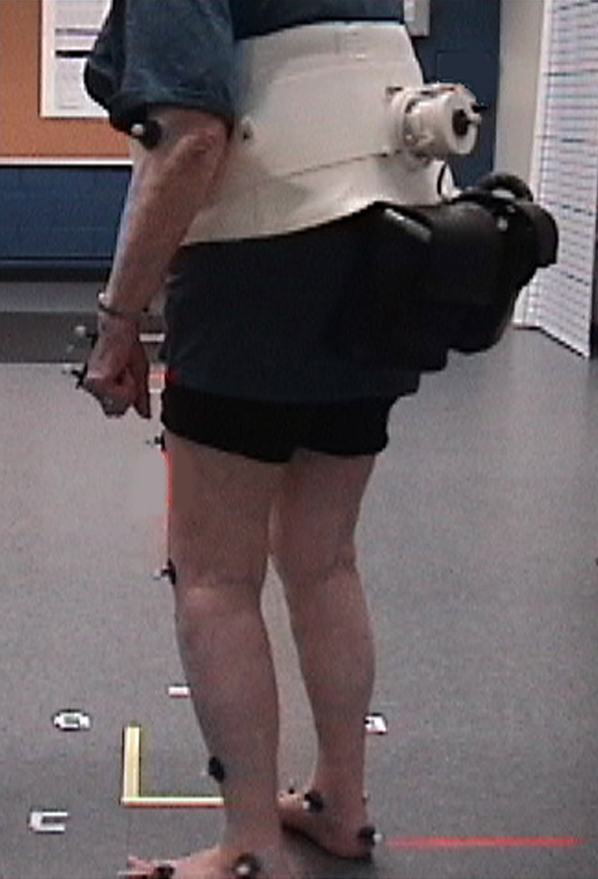
\includegraphics[width=0.40\textwidth]{sensors.png}
    \caption{\footnotesize Sensors fastened to an elderly person to detect mediolateral sway \cite{vibrotactileTiltFeedback}.}
\end{figure}

The collected data was sent to the computer in order to calculate the and compare the position of the trunk with the initial position. If trunk displacement was detected the subject was provided with feedback. The mentioned studies have primarily used vibration to give feedback about the trunk position, but light and sound was also utilized \cite{multiModualBiofeedback}.

\begin{figure}[h!]
  \centering
    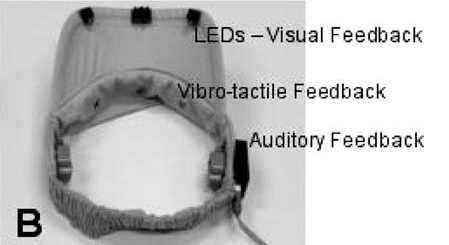
\includegraphics[width=0.80\textwidth]{biofeedback.png}
    \caption{\footnotesize Implementation of different types of biofeedback \cite{multiModualBiofeedback}.}
\end{figure}

These studies all conclude that giving vibrotactile and other types of biofeedback reduces the angular trunk displacement of patients. One of the studies showed that in some cases such systems influenced the balance of older adults \cite{multiModualBiofeedback}, while others showed improved control of mediolateral sway during gait and dynamic gait index, which are fall risk indicators in elders \cite{vibrotactileTiltFeedback}.

\subsection{Mobile fall detection systems}
Making biofeedback systems available for home users creates a new set of challenges. The sensors would have to be smaller and there would be the need for a computer to interpret the information gathered by the sensors. Smartphones are one example of portable computing units with small sensors that can be used for such purposes. Several attempts have been made to create fall detection systems using smartphone technology \cite{iFall, semiSupervisedFallDetection, mobilePhoneBasedFallDetection, detectionOfFalls}, all of these studies show positive results. Sadly there are no projects that focus on preventing falls through the use of smartphones and biofeedback, all of them focus on reacting to a fall, rather than preventing it.

The iFall \cite{iFall} project is a lightweight Android application designed to run in the background. It monitors the data from the smartphone’s accelerometer if the accelerometer data matches a predefined pattern it will assume a fall has occurred. When a fall is detected the user has a certain amount of time to get up again, this is to prevent false alarms when small falls occur or the phone is dropped. If the user does not get up, a prompt window is presented that the user has to respond to, if no response is registered an alarm will be triggered. 

\begin{figure}[h!]
  \centering
    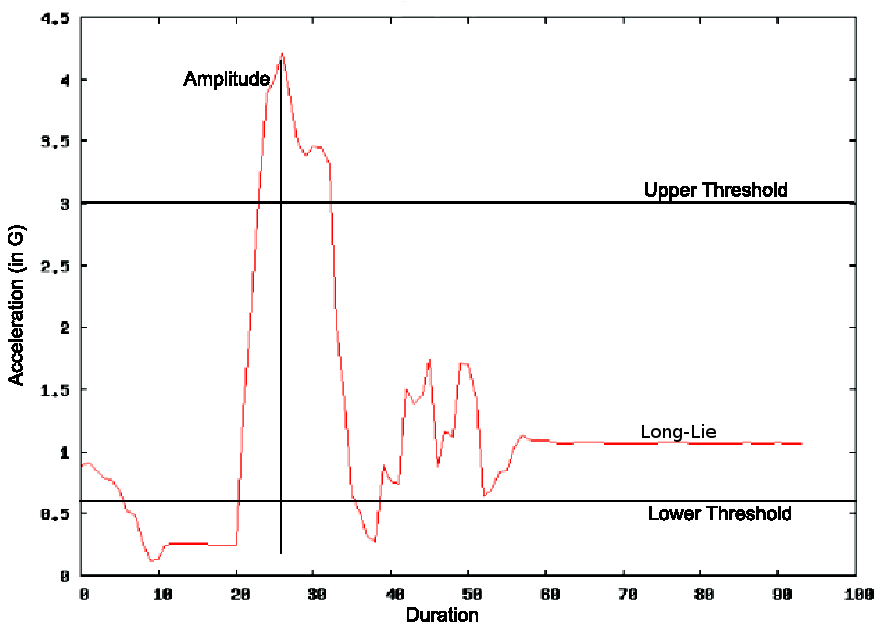
\includegraphics[width=0.80\textwidth]{patternGraph.png}
    \caption{\footnotesize An example of a classic fall. The accelerometer crossing the lower and upper amplitude  threshold followed by a long lie, recongnized this pattern as a fall.}
\end{figure}

One of the challenges the project faced was to alter and adapt the threshold depending on where the user carried the phone. Strapping it to the arm while running, or putting it inside a purse would generate more movement than on a belt clip or in a pocket. The application would identify patterns in the accelerometer data to decide where the user was most likely carrying his phone and set the appropriate thresholds. The project concludes that their software is viable and affordable, but the challenge is for the users to accept it and testing it out in the field to improve its usability.

\subsubsection{Sensor placement}
The PerFallID\cite{fallPrevention} project and a Taiwanese Android \cite{mobilePhoneBasedFallDetection} project have similarities to the previously mentioned iFall project, but do more research on how phone placement on the body affects the accuracy of their application. They perform a similar test by attaching the phone to chest, waist, and thigh and measuring the amount of false positive and false negatives. They reach different conclusions concerning the best placement for the smartphone; PerFallID concludes that the waist is the most accurate area, while the Taiwanese Android project concludes that the chest is the best location when using only one device with an accelerometer. The conclusions might come from the fact that different approaches and algorithms are used to detect falls. This could mean that there is no universal optimal position for the sensors to be located.

\begin{figure}[h!]
  \centering
    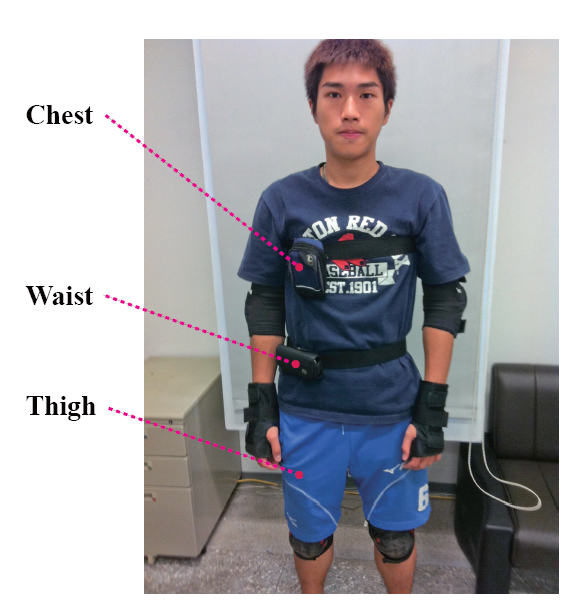
\includegraphics[width=0.60\textwidth]{phoneLocations.png}
    \caption{\footnotesize An example of the phone locations tested in the Taiwanese project.} 
\end{figure}

\subsubsection{Multiple sensors}
A common limitation for the papers that have been reviewed involve that only the smartphone is used as a sensors. The PerFallID implements an additional magnetic  sensor that is placed above the knee. By using the data from the magnetic sensor they are able to improve the accuracy of the application, backward and lateral falls gain a significant improvement with the additional sensor. The Environmental-Adaptive Fall Detection System \cite{fallDetectionWithExtraSensors} project takes advantage of 3 sensors, and the smartphone itself acts only as a hub. The sensors are located on the waist, left ankle and right ankle. Their solution is able to detect falls with 80\% accuracy in all kinds of situations, such as running, walking, ramp, standing still, and stairs. It seems to be the most complex solution so far, which makes battery life an interesting factor, but there is no mention of it in the paper.